\begin{figure}[t]
\centering
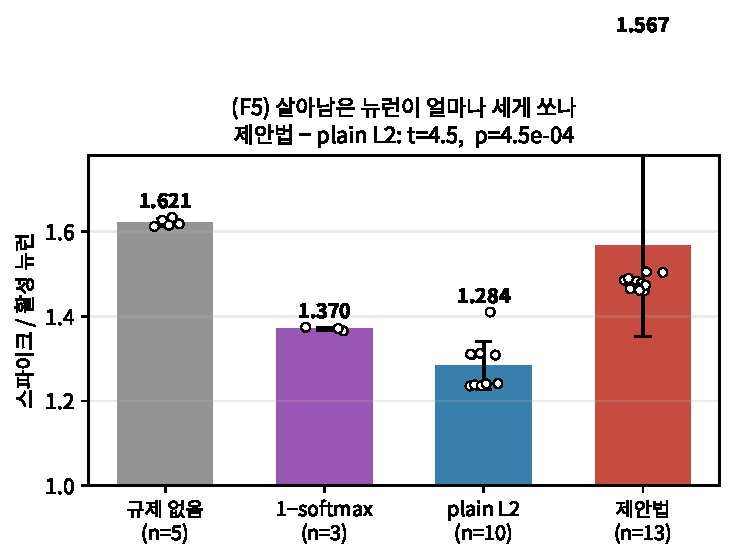
\includegraphics[width=\linewidth]{figures/f5_intensity_appendix.pdf}
\caption{Spikes per active neuron, ResNet-19/CIFAR-10, at the same
closest-landing pair used in Figure~\ref{fig:f2f3}. Bars are the
per-condition mean with individual runs overlaid; $n$ per condition is
given on the axis. Ours vs.\ Plain $L_2$: $t=10.5$, $p=8.4\times10^{-7}$.
As elsewhere in this section, the underlying active-neuron counts come
from \texttt{dead\_neuron\_ratio} measured over a 100-image batch -- not
a measurement of permanently silent neurons.}
\label{fig:f5_intensity}
\end{figure}
